% This is "sig-alternate.tex" V2.0 May 2012
% This file should be compiled with V2.5 of "sig-alternate.cls" May 2012
%
% This example file demonstrates the use of the 'sig-alternate.cls'
% V2.5 LaTeX2e document class file. It is for those submitting
% articles to ACM Conference Proceedings WHO DO NOT WISH TO
% STRICTLY ADHERE TO THE SIGS (PUBS-BOARD-ENDORSED) STYLE.
% The 'sig-alternate.cls' file will produce a similar-looking,
% albeit, 'tighter' paper resulting in, invariably, fewer pages.
%
% ----------------------------------------------------------------------------------------------------------------
% This .tex file (and associated .cls V2.5) produces:
%       1) The Permission Statement
%       2) The Conference (location) Info information
%       3) The Copyright Line with ACM data
%       4) NO page numbers
%
% as against the acm_proc_article-sp.cls file which
% DOES NOT produce 1) thru' 3) above.
%
% Using 'sig-alternate.cls' you have control, however, from within
% the source .tex file, over both the CopyrightYear
% (defaulted to 200X) and the ACM Copyright Data
% (defaulted to X-XXXXX-XX-X/XX/XX).
% e.g.
% \CopyrightYear{2007} will cause 2007 to appear in the copyright line.
% \crdata{0-12345-67-8/90/12} will cause 0-12345-67-8/90/12 to appear in the copyright line.
%
% ---------------------------------------------------------------------------------------------------------------
% This .tex source is an example which *does* use
% the .bib file (from which the .bbl file % is produced).
% REMEMBER HOWEVER: After having produced the .bbl file,
% and prior to final submission, you *NEED* to 'insert'
% your .bbl file into your source .tex file so as to provide
% ONE 'self-contained' source file.
%
% ================= IF YOU HAVE QUESTIONS =======================
% Questions regarding the SIGS styles, SIGS policies and
% procedures, Conferences etc. should be sent to
% Adrienne Griscti (griscti@acm.org)
%
% Technical questions _only_ to
% Gerald Murray (murray@hq.acm.org)
% ===============================================================
%
% For tracking purposes - this is V2.0 - May 2012

\documentclass{sig-alternate}
\usepackage[utf8]{inputenc}
\usepackage{graphicx}

\begin{document}
%
% --- Author Metadata here ---
% \conferenceinfo{WOODSTOCK}{'97 El Paso, Texas USA}
%\CopyrightYear{2007} % Allows default copyright year (20XX) to be over-ridden - IF NEED BE.
%\crdata{0-12345-67-8/90/01}  % Allows default copyright data (0-89791-88-6/97/05) to be over-ridden - IF NEED BE.
% --- End of Author Metadata ---

\title{Design and Implementation of an Appointment Scheduling Site for Innisfree Village}

%
% You need the command \numberofauthors to handle the 'placement
% and alignment' of the authors beneath the title.
%
% For aesthetic reasons, we recommend 'three authors at a time'
% i.e. three 'name/affiliation blocks' be placed beneath the title.
%
% NOTE: You are NOT restricted in how many 'rows' of
% "name/affiliations" may appear. We just ask that you restrict
% the number of 'columns' to three.
%
% Because of the available 'opening page real-estate'
% we ask you to refrain from putting more than six authors
% (two rows with three columns) beneath the article title.
% More than six makes the first-page appear very cluttered indeed.
%
% Use the \alignauthor commands to handle the names
% and affiliations for an 'aesthetic maximum' of six authors.
% Add names, affiliations, addresses for
% the seventh etc. author(s) as the argument for the
% \additionalauthors command.
% These 'additional authors' will be output/set for you
% without further effort on your part as the last section in
% the body of your article BEFORE References or any Appendices.

\numberofauthors{6} %  in this sample file, there are a *total*
% of EIGHT authors. SIX appear on the 'first-page' (for formatting
% reasons) and the remaining two appear in the \additionalauthors section.
%
\author{
% You can go ahead and credit any number of authors here,
% e.g. one 'row of three' or two rows (consisting of one row of three
% and a second row of one, two or three).
%
% The command \alignauthor (no curly braces needed) should
% precede each author name, affiliation/snail-mail address and
% e-mail address. Additionally, tag each line of
% affiliation/address with \affaddr, and tag the
% e-mail address with \email.
%
% 1st. author
\alignauthor
Bethany Connor\\
       \affaddr{University of Virginia}\\
       \email{bac5rc@virginia.edu}
% 2nd. author
\alignauthor
Robert Emerson\\
       \affaddr{University of Virginia}\\
       \email{roe2pj@virginia.edu}
% 3rd. author
\alignauthor
Will Emmanuel\\
       \affaddr{University of Virginia}\\
       \email{wre9fz@virginia.edu}
\and  % use '\and' if you need 'another row' of author names
% 4th. author
\alignauthor
Xavier Palathingal\\
       \affaddr{University of Virginia}\\
       \email{xvp2he@virginia.edu}
% 5th. author
\alignauthor
Domenic Puzio\\
       \affaddr{University of Virginia}\\
       \email{dvp5qd@virginia.edu}
% 6th. author
\alignauthor
Huiqing Zhang\\
       \affaddr{University of Virginia}\\
       \email{hz9cx@virginia.edu}
}
% There's nothing stopping you putting the seventh, eighth, etc.
% author on the opening page (as the 'third row') but we ask,
% for aesthetic reasons that you place these 'additional authors'
% in the \additional authors block, viz.

% Just remember to make sure that the TOTAL number of authors
% is the number that will appear on the first page PLUS the
% number that will appear in the \additionalauthors section.

\maketitle
\begin{abstract}
This paper describes an appointment scheduling system designed for Innisfree Village, a non-profit organization dedicated to adults with disabilities.  The previous system used for scheduling appointments was a handwritten calendar, which was messy, slow, and hard to keep records of.  This system was required to keep track of appointments, doctors, residents, and users of the system.  In addition, a car signout feature was added to help the organization manage a fleet of cars.  Due to the lack of internet in most houses at Innisfree, a mobile view was very important as that would be the primary method of access.  Through nine months of development, a functional system that met these requirements was designed, implemented, tested, and deployed to the organization.
\end{abstract}

% A category with the (minimum) three required fields
% \category{H.4}{Information Systems Applications}{Miscellaneous}
%A category including the fourth, optional field follows...
% \category{D.2.8}{Software Engineering}{Metrics}[complexity measures, performance measures]

% \terms{Web Application}

% \keywords{scheduling, web interface, Ruby on Rails}

\section{Introduction}
Innisfree Village is a non-profit organization located in Crozet, Virginia dedicated to providing a lifesharing community for adults with disabilities \cite{innisfree}. In this community, about 40 adults, known as co-workers, live and work alongside 20 long-term volunteer caregivers in houses of 4 co-workers and 2 caregivers. In addition to these full-time volunteers, there are around a dozen part-time volunteers and a dozen staff members providing more specialized knowledge and care. Throughout the day, residents participate in a variety of activities to contribute to the community, including cooking, gardening, woodworking, and weaving. Volunteers, who have committed to serving at the village for a year and a half, spend much of their time working together with their co-workers and helping meet their needs. Meanwhile, staff members are responsible for much of the administrative and maintenance work necessary to keep the community thriving.

As a full-time residential community, Innisfree Village is also responsible for scheduling medical appointments and ensuring co-workers can make these appointments. This is one of the main tasks for the staff, requiring one staff position, the medical coordinator, to be fully devoted to co-worker medical care, while also involving many others. Given that the 40 co-workers of Innisfree Village have varying disabilities and medical needs, ensuring all the necessary appointments have been made and can be attended is vital. Our work for them will focus on overhauling this scheduling system. The current system used for this is primarily pen and paper. When an appointment is made, the medical coordinator writes it on a large calendar in the main office, before recording it in Excel for reporting purposes. When a co-worker has an appointment, that co-worker’s volunteer caregiver is responsible for taking them to the appointment. These volunteers often need to reserve a shared car from the Village for this, so our work will include a component for this.

One of the major issues with this system is its lack of responsiveness. Not only is it exceedingly slow, as it requires several steps to simply record an appointment, but caregivers are rarely able to make follow-up appointments in the doctor’s office, as it also requires several phone calls between the medical coordinator and the doctor to schedule an appointment. The current system also requires appointments to be entered twice, increasing the secretarial load required, and increasing the possibilities of errors. It also makes it hard to generate reports for specific houses or residents, as Excel does not provide the same features as a full database system. Finally, it is not simple for the medical coordinator to remind caregivers about upcoming appointments. Since all appointments are recorded on the calendar, the medical coordinator writes paper reminders for each caregiver, and has to hope the caregiver will check their mailbox in time.

Our system has significantly increased the efficiency of Innisfree's scheduling system. Volunteers can now schedule appointments by filling out a form on our website, which will then display under the calendar and upcoming appointments, which can be filtered by houses and specific residents. We have also implemented a mobile interface, so users can quickly view this information from anywhere using their phone. Our system also allows for easy management of residents, houses, volunteers and cars through each of the corresponding pages. Cars can be reserved through our reservation page, where volunteers and staff can see which cars are available at what times. In order to further optimize scheduling time, volunteers can quickly make follow-up appointments from the page after viewing the appointment. Email reminders for each appointment are sent to the assigned volunteer if desired, as well as to the medical coordinator on a weekly basis. Our system also provides a dynamic report generation system, whereby the staff can generate custom filtered reports for all data stored within the systems.

This system was designed through the Service Learning Practicum at the University of Virginia.  This program allowed students to work directly with a non-profit customer on a project that would have real usefulness and application for their organization.  

\section{Related Work}
There are several applications that were discussed with Innisfree Village as possible solutions.  The first one discussed was mainstream online scheduling options such as Google Calendar. While our system was eventually modeled on the view of Google Calendars, this kind of calendar was too generic for what our customers wanted.  It does not allow for the management of residents, doctors, volunteers, or cars, there are few user levels, and they are difficult to filter.  In addition, these calendars are made to be managed by one person and viewed by many, which did not fit in with the needs of this system. Finally, these applications do not allow data to be exported in a report friendly format, something our customer required.
	
Another scheduling option included desktop clients, such as Outlook, as these also have a developed calendar.  However, programs like this do not fit with the way volunteers would use the site, which is mostly on their cell phones and would not support car sign-out features.  As with Google Calendar, there is no way to manage user levels, or reserve cars.

\section{System Design}

\subsection{Users}

\subsubsection{Users Model}
The user model lists all of the attributes for system users. This includes the user’s name, email, house, email preferences, and admin status, as well as several fields automatically created by Ruby on Rails. Since we used the Devise gem \cite{devise} for user authentication, it generates and automatically fills fields for the user's password, password reset, and other login information. The user's name, email and password are all required fields when a new user is created. The house field is not explicitly required, but is always filled out at account creation time. As there is a one-to-many relationship between houses and users, where each house has many users and each user has one house, when the house field of a user is changed it is validated against the houses in the database to ensure that house actually exists.

\subsubsection{Viewing, Creating, Editing, and Deleting Users}
The users are displayed in two places. The first is a user directory, accessible to all users, where a user can look up the house, email address, or phone number of another user. Users can also edit their own profile from this page. The second user display an administrative interface that only administrator users can access. Here, administrators can mark other users as administrators or as medical coordinators, turn user emails on and off, edit user profiles and delete users.

\begin{figure}
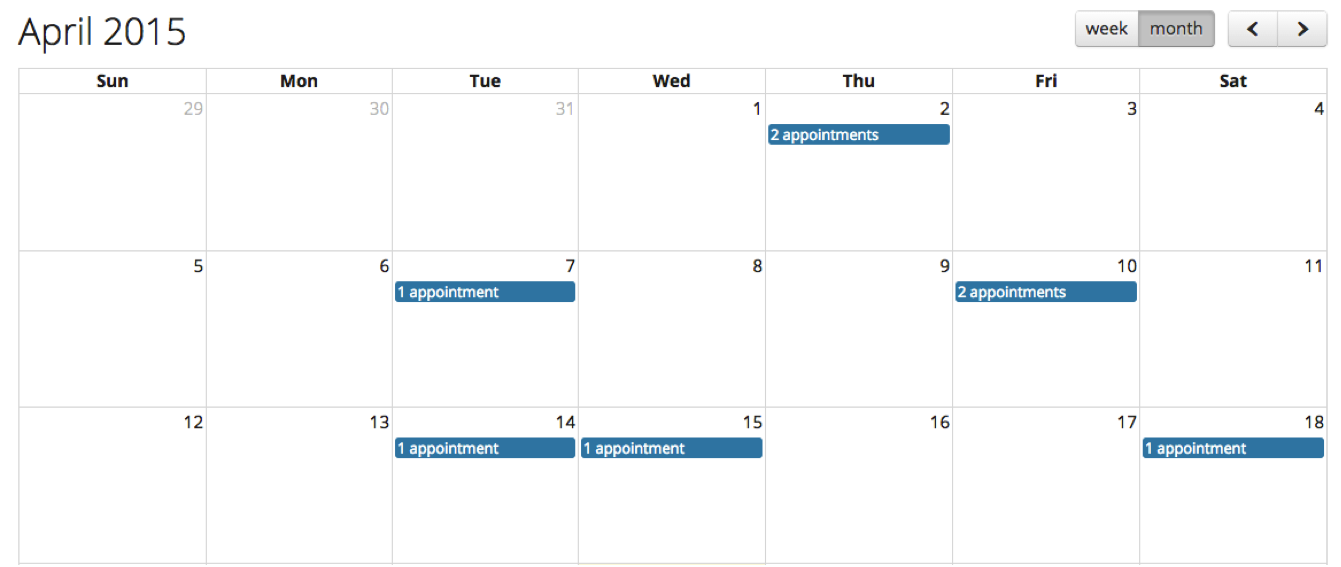
\includegraphics[scale=0.4]{Calendar}
\caption{A screenshot of the calendar view of appointments.  Each day shows the number of appointments scheduled.  Clicking on the day will bring up a modal window listing those appointments.}
\end{figure}

\subsection{Appointments}

\subsubsection{Appointments Model}
The appointments model contains attributes for the resident, the doctor, the date, the time, the volunteer assigned to the appointment, the appointment type, a notes section, whether the appointment has been canceled and the Ruby on Rails generated ID, created-at, and updated-at fields.  In order to create an appointment, the resident ID (from the Resident table), the doctor ID (from the Doctor table), the appointment type, the date, and the time must be specified.  The notes field user id of the volunteer assigned to the appointment defaults to NULL and the canceled field defaults to false.  The fields for ID, created-at, and updated-at are all purely managed by Ruby on Rails. 

In addition, the customer requested that we have a way of tracking updates to an appointment.  For this, we used the Rails gem PaperTrail. \cite{papertrail}  This created a separate table named versions that kept track of each of these events for any model we marked as being tracked.  Namely, this table contains a copy of the object as well as the type of the object.

\subsubsection{Viewing, Creating, Editing, and Deleting Appointments}
The appointments are displayed on the landing page of the site in both a list and calendar format.  In the calendar view, displayed using the FullCalendar Rails gem \cite{fullcalendar}, we chose to only show the number of appointments on that given day in an effort to reduce clutter (see Figure 1).  However, each day has the option to click on it to see the full list of appointment on that day.  The list view on the landing page is a paginated list of the next ten appointments.

Creating appointments can be done by both administrators and volunteers.  There is a button above the appointments display to create a new appointment.  This brings up a form that has fields for all fields of the appointments model except the Rails managed fields and the ``canceled" field.  All fields are drop-down menus except for the date, time, and notes fields.  The items in these drop-down menus are pulled straight from other tables of the database, and, as the only table volunteers can create entries into is the appointments table, are managed by the admin of the site.

As the project progressed, we realized that outright deleting an appointment did not constitute the same action as canceling one.  Therefore, we added an option to cancel an appointment.  These appointments then still appeared anywhere they would have before cancellation but with a strike-through.  This allowed for better communication between the various employees of the Village and to demonstrate that an appointment had indeed been made.  Volunteers and admin can both cancel an appointment (and un-cancel it if the cancellation was done in error) but only administrators can outright delete an appointment.      

\subsection{Residents}
\subsubsection(Residents Model)
The residents model contains attributes for each resident's name, house, a notes field, and created and last updated timestamps. Each resident is required to have a name upon creation. Residents belong to the house in which they live. Each resident may only be assigned to one house, while any given house will have many residents.

\subsubsection(Viewing, Creating, Editing, and Deleting Residents)
Although all users can view residents through the houses page, only admins can create and delete residents. Admins can edit all residents as well, while volunteers can only edit residents within their house. Admins can view the resident management page, which shows the name, house, notes, as well as links to show, edit, and delete for each resident. 

\begin{figure}
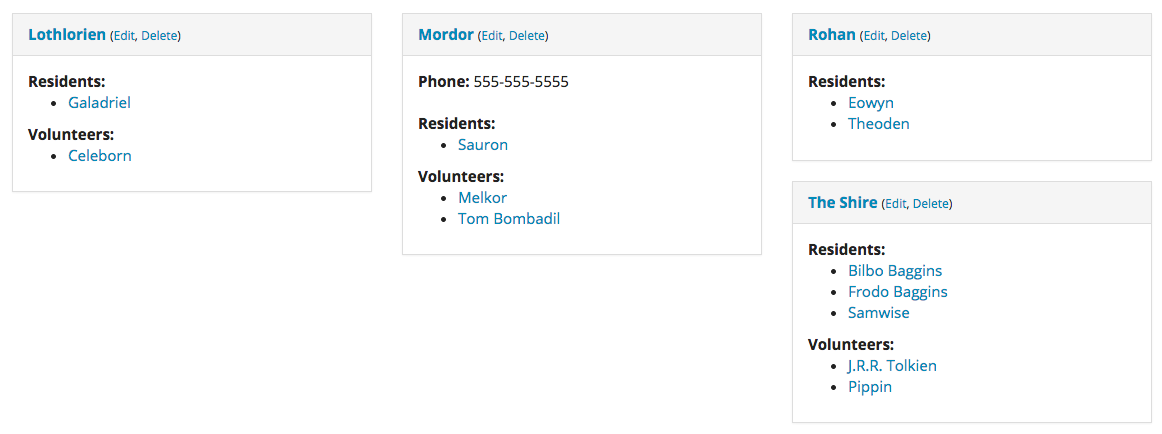
\includegraphics[scale=0.2]{Houses}
\caption{A screenshot of the house layout with residents and volunteers listed.}
\end{figure}

\subsection{Houses}
Houses are a fairly simple part of our application. Each house has a name that must be given when it is created, as well as an optional phone number that can be used to reach that house. Each house also has several residents and users, and is used to validate entered values in those models.  In the display, the houses are shown with the residents and users (see Figure 2). Houses serve as a way to control user access to residents and appointments, as non-admin users can only edit residents and appointments in their associated house. Administrative users are exempt from these controls and are also the only users able to create and delete houses.

\subsection{Doctors}

\subsubsection{Doctors Model}
The doctors model contains attributes for each doctor’s name, address, phone number and doctor type. All doctors must at least have values for their names. 

\subsubsection{Creating, Viewing, Editing and Deleting Doctors}
Only admins can create, edit and delete doctors. In order to create a new doctor, the user must enter the name of that doctor. Users can view the information about each doctor by clicking on their names. Users can also click on each doctor’s address and they will be redirected to location of that address on Google maps. 

\begin{figure}
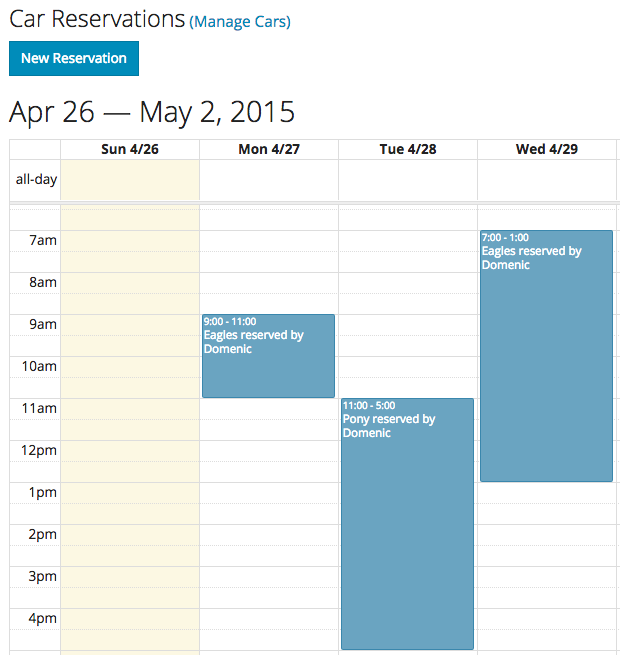
\includegraphics[scale=0.4]{Cars}
\caption{A screenshot of the cars reservation system.}
\end{figure}

\subsection{Cars}
On the cars page, each car has a name. Only admins can edit car names and create or delete cars. All users can make new reservations for cars. After users enter the date and time range for their reservation, they can click on “See Available Cars” to see if there are any cars available. The system will prompt users with warning messages if the time range is invalid or no cars are available. Otherwise, the user can choose one of the available cars, enter the purpose of car reservation in a text box and successfully create a new reservation. All the existing car reservations will be shown in a calendar (see Figure 3). Users can click on that reservation on the calendar, see details about that reservation and delete the reservation if they desire. 

\begin{figure}
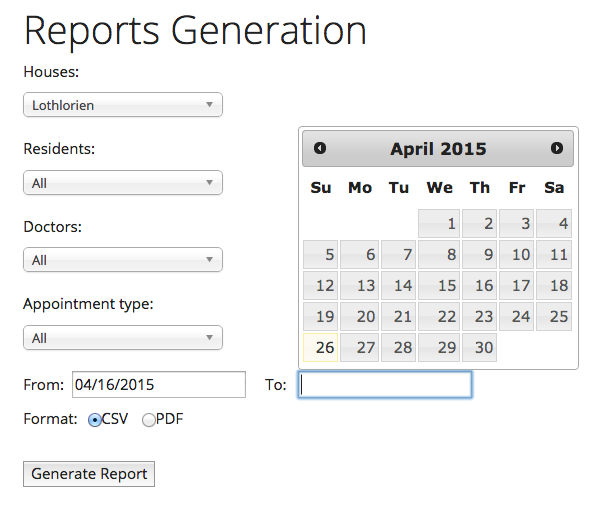
\includegraphics[scale=0.4]{ReportGeneration}
\caption{A screenshot of the form used to generate pdf reports.}
\end{figure}

\subsection{Reports}
On Reports page, admins can generate reports for the complete record of residents' appointments. They have the option to filter each report's content by houses, residents, doctors, appointment type and date range (see Figure 4). Two types of formats are available for these reports, CSV and PDF. Users can choose one of the format before they generate the report. CSV files can be easily imported into Excel and other data management software for further editing. PDF files have logo of Innisfree Village in the heading and they are well-formatted with clear headings and tables. Users can easily read them and print them out for filing purposes. 

There is a second type of reports that users can generate in Houses page, Home page, Doctors page and Users page. Users can generate a CSV file that includes all the context that are currently displayed on that particular page. For example, if the user chooses to generate this type of CSV report for doctors, that user will go to Doctors page and click on "Download as CSV" and download a CSV file that contains all the information including every doctor's name, address, doctor type and phone number. 

\subsection{E-mail Notifications}
At the beginning of development, e-mail notifications were limited to simply e-mailing volunteers the morning of appointments that were assigned to them.  However, as the project progressed, we added more notifications including weekly digests, reminders to schedule appointments, and the option to remind volunteers of a specific appointment.  In addition, who was sent these notifications was changed; instead of only being to the volunteer assigned, it was sent to the volunteers of the house of the applicable resident.

In order to send e-mails, we used ActionMailer \cite{actionmailer}, which comes with Rails.  For each type of e-mail we sent, we wrote a new function in NotificationMailer, which was our extension of ActionMailer.  Then, in our User model, we defined who these functions were sent to.  For example, we have a method called send\_weekly\_digest.   This iterates through the users, selects the ones that are medical coordinators (only medical coordinators get the weekly digest), then calls the weekly\_digest method in NotificationMailer.  A schedule defined in config/schedule.rb defines how often to call certain functions; for example in the case of the weekly digest, it is sent at 6am on every Sunday.  Other types of notifications are triggered by an action on the site and are therefore not scheduled in schedule.rb. 

\subsection{Mobile View}
One of the final customer requirements for our project was a mobile interface for creating, editing and viewing appointments. This requirement influenced the entire site design, as page elements were laid out in a manner that would feel intuitive on many different screen sizes. It also lead us to design a custom FullCalendar view that featured vertically arranged appointments, instead of a horizontal list or the calendar grid, specifically for small screened devices like smartphones or netbooks.

\section{Results}
% 27 appointments in March 2015
At the end of our initial development cycle, the customer began using the scheduling system.  This included them putting in real data.  For the next ten weeks, development occurred alongside the customer using the system, so bugs were found quickly and the customer quickly learned new features of the system.  Then a six week transition period began where development halted and the customers continued to use the system.

In April of 2015, the last full month prior to this writing, 18 appointments were entered.  Similarly, 27 were scheduled for March and 24 were scheduled in February, with the maximum number of appointments per day hitting five.  Assuming that the number of appointments did not change with the introduction of this system, the staff at Innisfree Village had to keep track of over 20 appointments on a paper calendar.  This included appointments that might move or be canceled.  In contrast, these appointments are now all in one place, in a system that is more scalable as the non-profit grows, changes can be made easily, and communication between the volunteers and the administration is more streamlined.

According to our customer, this system makes their work twice as fast.  Using the number of appointments scheduled above, an average of 23 appointments per month.  Let's say, just for simplicity, each appointment took two minutes to schedule and now takes one (the one minute for scheduling is backed up by tests).  This means, that 4.6 hours are saved each year from simply entering appointments into the calendar.  These are hours that could instead be used to work with the residents or work to expand the village.

In addition, our customer needed to create reports from an Excel spreadsheet.  All the appointments were documented in this spreadsheet and when reports need to be generated, it required finding the relevant information and compiling it into a document.  Now this is almost completely eliminated.  The data entry is the same as recording the appointments and report generation takes less than a minute with a simple form, whereas it might have taken several minutes before.  If it even saves four minutes per resident, over forty residents, this will have 2 hours and 40 minutes over the course of the year (reports aren't generated much more than once per year).  

Based on the high use of this system by the customer, we believe that this project was a success.  We achieved all of our requirements laid out for us at the beginning of the project and were adaptable to changes in these requirements.

\section{Challenges}
Although we have met all the required and desired features, there are still some challenges left. Some users might need help understanding and using the system at first and confusions might occur during their use of the system. Maintaining the website and fixing hidden bugs might be a challenge for Innisfree Village staff members in the future. Some current functions might lack additional features that could make the system more user-friendly. More functions might be needed when the structure or organization of Innisfree Village changes. We believe that maintaining a website is a dynamic process during which new problems should be solved as they occur. New challenges will also occur during the process and we should prepare our system for such challenges.

\section{Future Work}
There are several logical extensions of our work. The first is a calendar for the volunteer shifts. This calendar could be used to display when certain volunteers were working or had their day off. While our customer indicated this would be beneficial, they believed it to be relatively unimportant, especially when compared to appointment and car management. Making the appointment calendar more descriptive could also better the system, by more fully presenting appointment information. This could be achieved by separating the different appointments scheduled for each day, either by resident, appointment, doctor, or location. The final extension we considered is a dedicated mobile application for smartphones and tablets, as this would increase usability on a variety of mobile platforms. As mobile browsers all render elements differently, we cannot be sure that our site is usable on every device without extensive testing with phones and tablets from every manufacturer. As this is unrealistic, a mobile app could help us simplify our testing and optimize our site a few major platforms.

\section{Conclusion}
Over the course of nine months in the Service Learning Practicum, we designed, implemented, and tested this system.  With the help of our customer, we believe we designed a functional system that fit their specific needs and can scale with their organization.  It also allowed them to keep all data in one place and backup their data as necessary.  With more time, this project could be extended to provide even more convenience, but, given the timeframe and expectations of the project, we provided a functional system that met requirements.  

%ACKNOWLEDGMENTS are optional
\section{Acknowledgments}
We would like to thank Monika, Emily, Wes, and Eric from Innisfree Village for all their help with designing and testing this system.
 

%
% The following two commands are all you need in the
% initial runs of your .tex file to
% produce the bibliography for the citations in your paper.
\bibliographystyle{abbrv}
\bibliography{sigproc}  % sigproc.bib is the name of the Bibliography in this case
% You must have a proper ".bib" file
%  and remember to run:
% latex bibtex latex latex
% to resolve all references
%
% ACM needs 'a single self-contained file'!
%
\end{document}
